% Created 2026-04-23 Thu 12:08
% Intended LaTeX compiler: lualatex
\DocumentMetadata{lang = en-US,pdfversion = 2.0,pdfstandard = ua-2,tagging = on,tagging-setup = {math/setup=mathml-SE},}
\documentclass[11pt]{article}
\usepackage{amsmath}
\usepackage{fontspec}
\usepackage{graphicx}
\usepackage{longtable}
\usepackage{wrapfig}
\usepackage{rotating}
\usepackage[normalem]{ulem}
\usepackage{capt-of}
\usepackage{hyperref}
\usepackage[margin=1in]{geometry}
\usepackage{fontspec}
\usepackage{verbatim, multicol, tabularx,}
\usepackage{amsmath, amsthm, amssymb, stmaryrd, latexsym, bm, listings, qtree}
\usepackage{framed}
\usepackage{xcolor,colortbl}
\usepackage{media9}
\usepackage[export]{adjustbox}
\usepackage{algorithm}
\usepackage[noend]{algpseudocode}
\usepackage{tikz,pgfplots}
\usetikzlibrary{shapes.geometric}
\let\oldquote=\quote
\let\endoldquote=\endquote
\colorlet{shadecolor}{cyan!15}
\renewenvironment{quote}{\begin{shaded*}\begin{oldquote}}{\end{oldquote}\end{shaded*}}
% From https://tex.stackexchange.com/questions/7032/good-way-to-make-textcircled-numbers
\newcommand*\circled[1]{\tikz[baseline=(char.base)]{\node[shape=circle,draw,inner sep=2pt] (char) {#1};}}
\DeclareMathOperator*{\argmin}{arg\!min}
\DeclareMathOperator*{\argmax}{arg\!max}
\lstset{frame=tb, aboveskip=1mm, belowskip=0mm, showstringspaces=false, columns=flexible, basicstyle={\scriptsize\ttfamily}, numbers=left, frame=single, breaklines=true, breakatwhitespace=true}
\hypersetup{colorlinks=true,urlcolor=blue}
\usepackage{tagpdf}
\tagpdfsetup{activate-all}
\tagpdfsetup{math/alt/use}
\usepackage{polyglossia}
\setdefaultlanguage[variant=en-US]{english}
\author{Christopher Simpkins}
\date{Kennesaw State University}
\title{Artificial Intelligence\\\medskip
\large Markov Decision Processes (AIMA 17)}
\hypersetup{
 pdfauthor={Christopher Simpkins},
 pdftitle={Artificial Intelligence},
 pdfkeywords={},
 pdfsubject={Artificial Intelligence Markov Decision Processes (AIMA 17)},
 pdfcreator={Emacs 30.2 (Org mode 9.7.11)}, 
 pdflang={English}}
\begin{document}

\maketitle
\section{Sequential Decisions}
\label{sec:org868bbbb}


In \textbf{sequential decision problems}, the agent's utility depends on a sequence of decisions.

Sequential decision problems incorporate utilities, uncertainty, and sensing, and include search and planning problems as special cases.

\begin{itemize}
\item Markov decision processes (MDPs)
\item \$k\$-Armed bandits
\item Partially observable MPDs (POMDPs)
\end{itemize}
\section{Worlds}
\label{sec:orga0b7788}


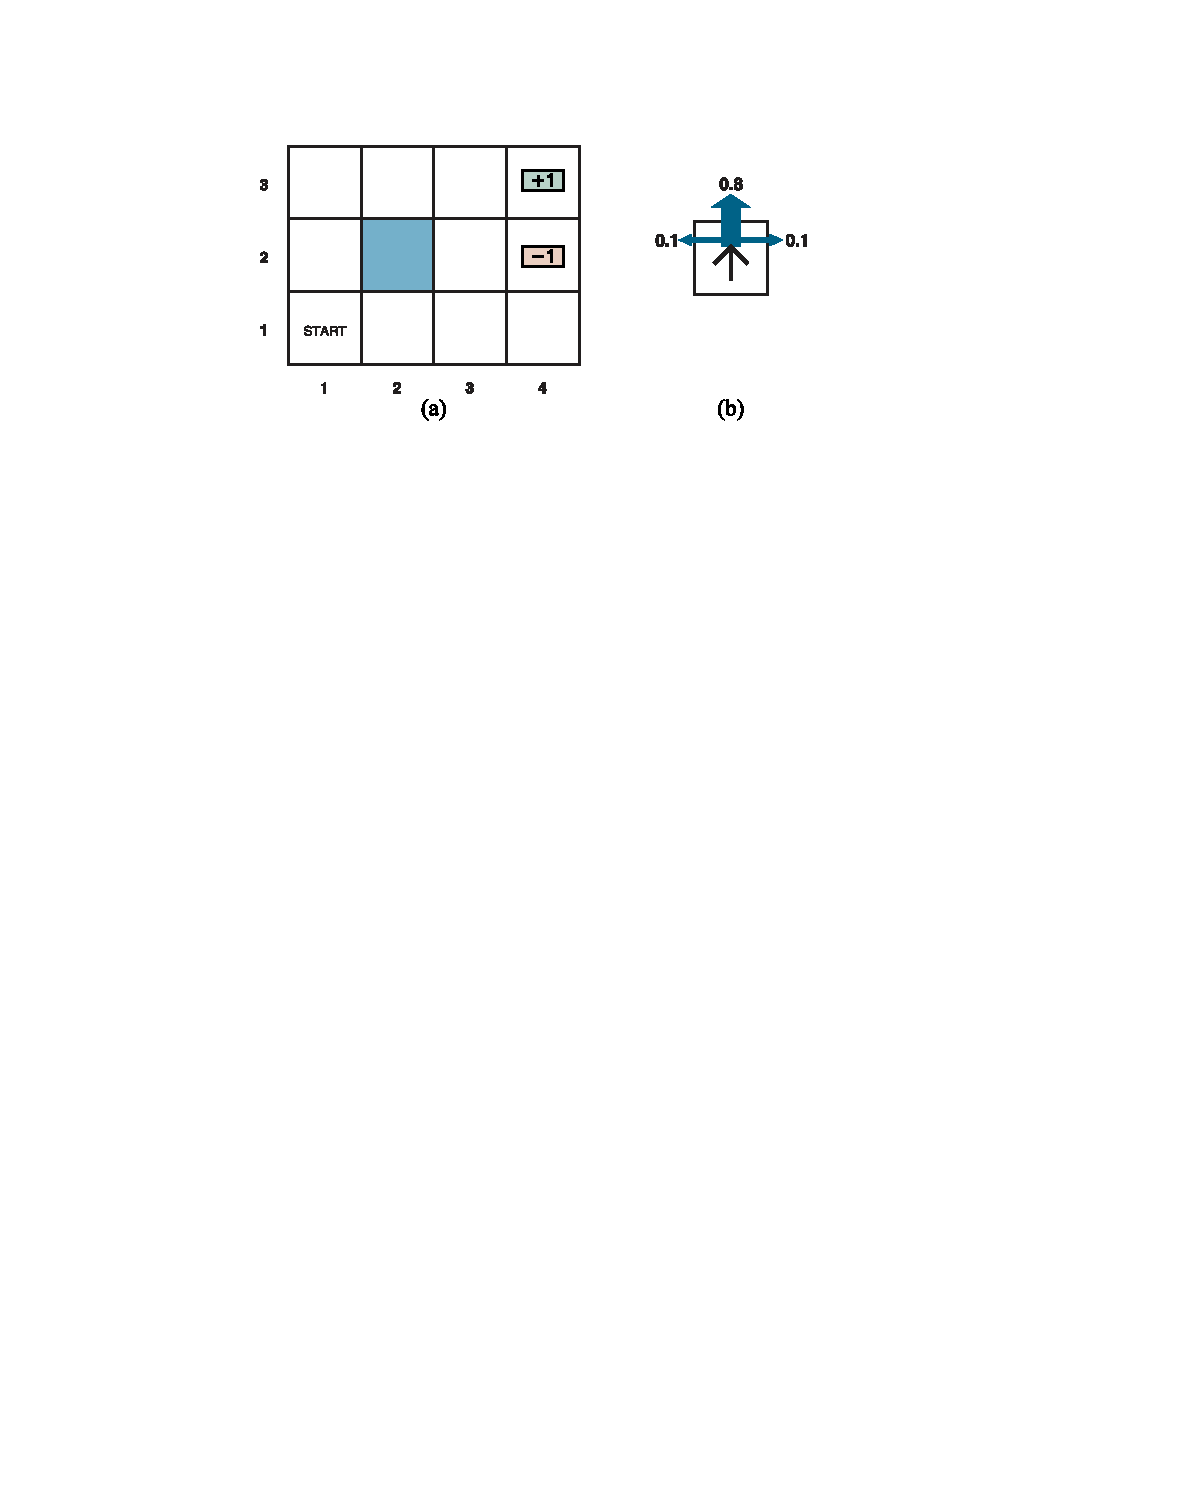
\includegraphics[alt={aima fig 17_01 4x3 grid world stochastic actions},width=0.75\linewidth]{aima-fig-17_01-4x3-grid-world-stochastic-actions.pdf}
\section{Markov Decision Processes (MDPs)}
\label{sec:orge83ec8e}

A Markov decision process (MDP) is a 4-tuple \(\left( S, A, Pr(s' \mid s, a), R(s) \right)\), where

\begin{itemize}
\item \(S\) is a set of states,
\item \(A\), or \(Action(s)\) is a set of actions, and
\item \(Pr(s' \mid s, a)\) is a transition function giving the probability that executing action \(a\) in state \(s\) will result in \(s'\).

\begin{itemize}
\item Many authors use \(T(s, a, s')\)
\end{itemize}

\item \(R(s, a, s')\) is the reward the world provides to an agent for arriving in state \(s'\) after executing action \(a\) in state \(s\), bounded by \(\pm R_{max}\)

\begin{itemize}
\item Many authors use \(R(s')\), which is easier to think about -- the reward for arriving in state \(s'\) regardless of the \(s, a\) pair in the previous time step.
\end{itemize}
\end{itemize}

Some definitions of MDPs include an initialization function, \(I(s)\), which specifies the probability the the agent will start in some state \(s \in S\), others specify a particular state \(s_0\) from \(S\) as the start state.
\section{MDP Solutions: Policies}
\label{sec:orgbd72963}

Due to stochastic action results, fixed plans don't work.  We need a function that returns a recommended action for every state.  Such a function is called a \textbf{policy}:

\begin{equation*}
\pi(s)
\end{equation*}

The policy can also be stochastic, \(\pi(a \mid s)\), but for now we'll assume deterministic policies.

By the maximum expected utility principle, for a policy to be optimal the action it recommends for each state must have the highest \textbf{value} among all the action choices in that state.

\begin{quote}
The book uses state/action \textbf{utility} instead state/action \textbf{value}, but this is inconsistent with the book's previous definition of utility and its relationsip to preformance measures, and it's inconsistent with the terminology used by the reinforcement learning community, which is where this is headed.  So we'll use \textbf{value} instead of \textbf{utility}.
\end{quote}
\section{Values and Trajectories}
\label{sec:org1254b20}

Since we're in the realm of sequential decisions, the value of an action depends on the \textbf{trajectory} -- the sequence of states and actions -- to which it leads.

\begin{quote}
Here again, we depart from the book's terminology.  The book uses \textbf{history}, but the reinforcement learning community uses the term \textbf{trajectory}, \(\tau\), so we'll use \(\tau\).  We'll also add reward to the trajectories, in line with reinforcement learning literature.
\end{quote}

An experience sequence through an MDP is called a \textbf{trajectory}:

\begin{equation*}
\tau = s_0, a_0, r_1, s_1, a_1, r_2, s_2, a_2, r_3, \dots
\end{equation*}

And the values in an MDP are defined in terms of a trajectory:

\begin{equation*}
V_{\tau}(s_0, a_0, r_1, s_1, a_1, r_2, \dots, s_{t-1}, a_{t-1}, r_t)
\end{equation*}

We'll define these values after we learn about rewards.
\section{Goals and Rewards}
\label{sec:org33f2234}

The purpose or goal of the agent is formalized in terms of a special signal, called the reward, passing from the environment to the agent.

\begin{itemize}
\item At each time step, the reward is a simple number, \(R_t \in \mathbb{R}\).
\item The agent’s goal is to maximize the total amount of reward it receives.

\begin{itemize}
\item This means maximizing not immediate reward, but cumulative reward in the long run.
\end{itemize}
\end{itemize}

We can clearly state this informal idea as the reward hypothesis:

\begin{quote}
All of what we mean by goals and purposes can be well thought of as the maximization of the expected value of the cumulative sum of a received scalar signal (called reward).
\end{quote}

So we represent goal states as the states giving the highest reward, with other states giving less reward according to some structure, which we'll discuss later.  First, how do we use these rewards to determine values, which is what we need to derive policies \ldots{}
\section{Returns and Finite Time Horizons}
\label{sec:org3094a04}

As the agent traverses an MDP along some trajectory, it collects reward on each state transition.  The total reward collected in a trajectory is called the \textbf{return}, \(G\).  The simplest way to calculate return is simple addition.  For a trajectory of length \(T\):

\begin{equation*}
G_t \doteq r_{t+1} + r_{t+2} + \cdots + r_T
\end{equation*}

With a finite horizon, there is an end time after which nothing happens, so if the end is time \(N\):

\begin{equation*}
V_{\tau}(s_0, a_0, r_1, s_1, a_1, \dots, r_{N+k}, s_{N+k}) = V_{\tau}(s_0, a_0, r_1, s_1, a_1, \dots,  r_N, s_{N})
\end{equation*}

Finite time horizons lead to \textbf{nonstationary} policies, i.e., policies that differ based on time.  Consider that happens if \(N=3\) vs \(N > 6\) in our \(4 \times 3\) grid world:



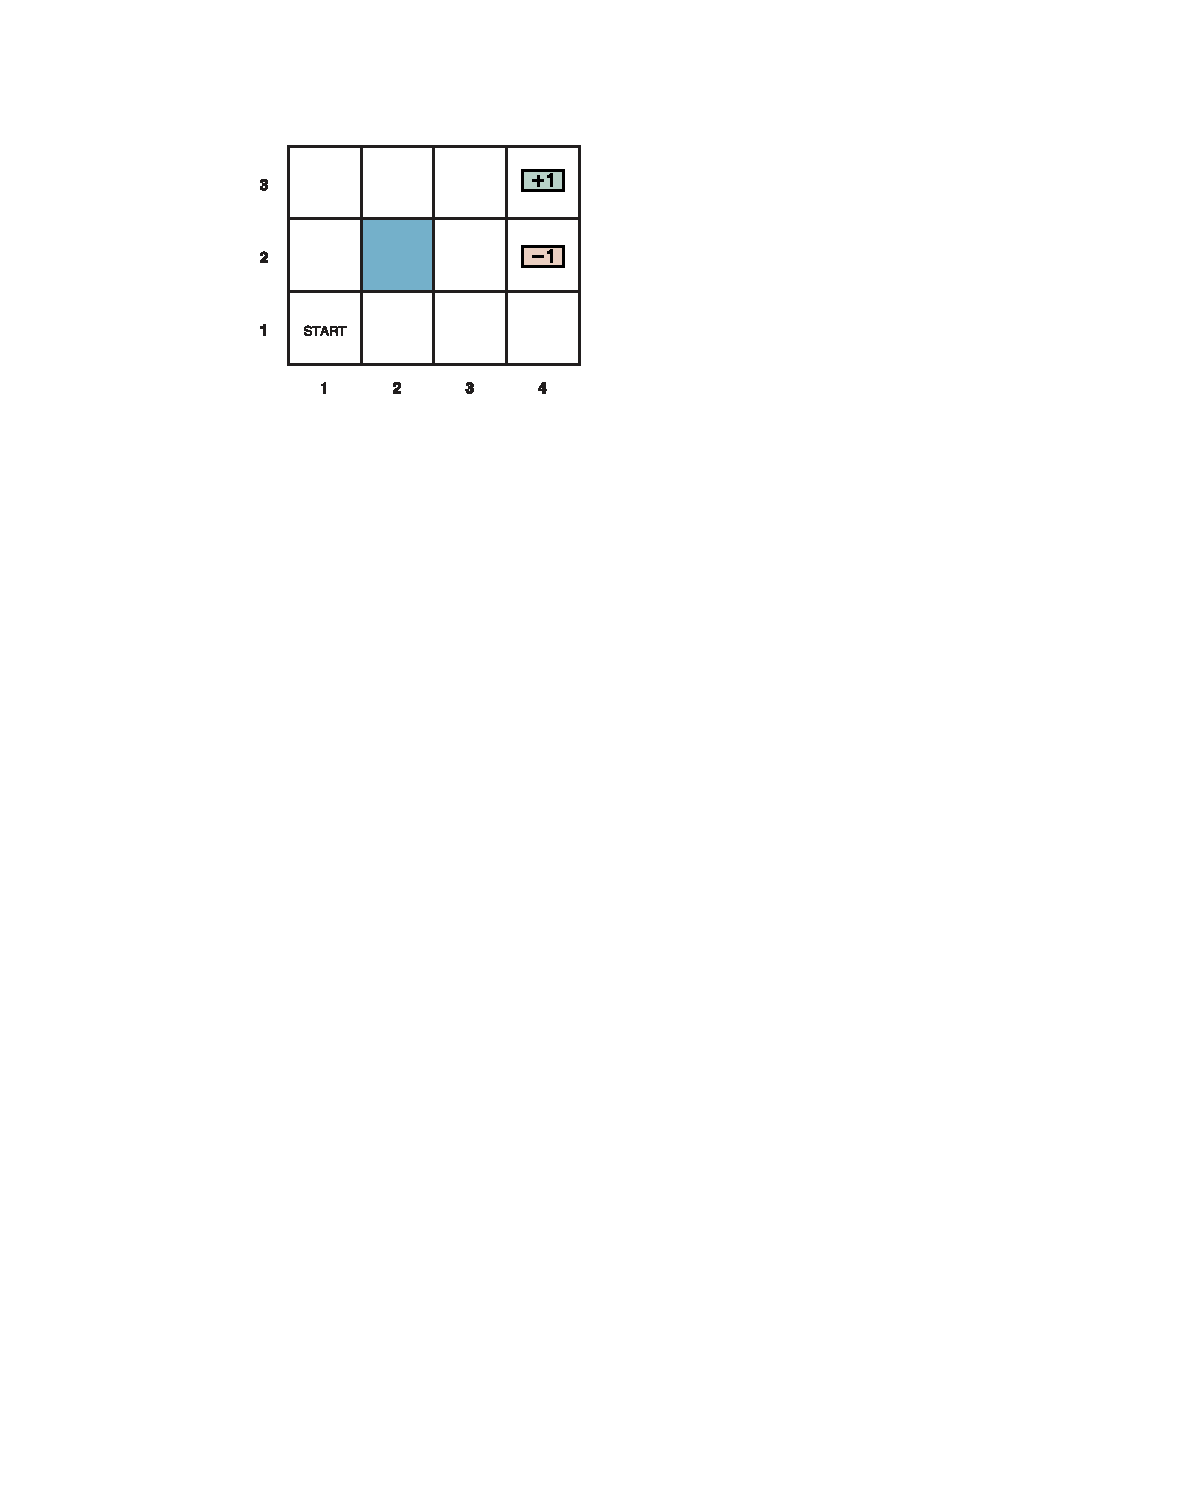
\includegraphics[alt={aima fig 17_01_a 4x3 grid world},width=0.75\linewidth]{aima-fig-17_01_a-4x3-grid-world.pdf}


The shorter time horizon forces the agent to risk ending up in state (4, 2), whereas the longer horizon allows the agent to take the long way around to the goal state.
\section{Infinite Horizon Return}
\label{sec:org39ab1cd}

An infinite horizon gives us a \textbf{stationary} policy, because there is no time limit influencing the decision.  From the current time step \(t\):

\[
G_t = r_{t+1} + r_{t+2} + \cdots + r_{t+k+1} =  \sum_{k = 0}^\infty \gamma^k r_{t+k+1}
\]

\(\gamma\) is the \textbf{discount factor} which says how much we discount future rewards.  With \(\gamma < 1\) it decays toward zero.

If rewards are bounded by \(\pm R_{max}\) and \(0 \le \gamma < 1\), then, using the standard sum of an infinite geometric series.

\begin{equation*}
V_{\tau}(s_0, a_0, r_1, s_1, a_1, r_2, \dots, s_{t-1}, a_{t-1}, r_t, s_t) = \sum_{t=0}^{\infty} \gamma^t R(s_t, a_t, s_{t+1}) \le \sum_{t=0}^{\infty} \gamma^t R_{max} = \frac{R_{max}}{1-\gamma} \tag{17.1}
\end{equation*}

So the values of infinite trajectories are finite.

\begin{itemize}
\item We will use inifinite horizon models.
\item We can convert any finite horizon model into a infinite one by making terminal states \textbf{absorbing states}, which include a single action that loops to the absorbing state and gives zero reward.
\end{itemize}
\section{State Values and Optimal Policies}
\label{sec:orgaab828c}

The expected value of executing \(\pi\) in starting in state \(s\) is:

\begin{equation*}
V^{\pi}(s) = \mathbb{E} \left[ \sum_{t=0}^{\infty} \gamma^t R(s_t, \pi(s_t), s_{t+1}) \right]
\end{equation*}

The expectation \(\mathbb{E}\) is with respect to the probability distribution over state sequences
determined by \(s\) and \(\pi\).  Remember that \(\pi(s_t)\) returns an action \(a_t\).  One or more policies, \(\pi^*\), will have the highest of all values.

\begin{equation*}
\pi^*(s) = \argmax_{a \in A(s)} \sum_{s'} Pr(s' \mid s, a) \left[ R(s, a, s') + \gamma V(s') \right] \tag{17.4}
\end{equation*}

The value of a state is the expected reward for the next transition plus the discounted utility of the next state, assuming that the agent chooses the optimal action. That is, the utility of a state is given by

\begin{equation*}
V(s) = \max_{a \in A(s)} \sum_{s'} Pr(s' \mid s, a) \left[ R(s, a, s') + \gamma V(s') \right] \tag{17.5}
\end{equation*}

This is the \textbf{Bellman equation}, which is the basis of the value iteration algorithm we'll see soon.
\section{Bellman Equation Example}
\label{sec:org42d8239}




What is the optimal action in state (1, 1) given the following state values?





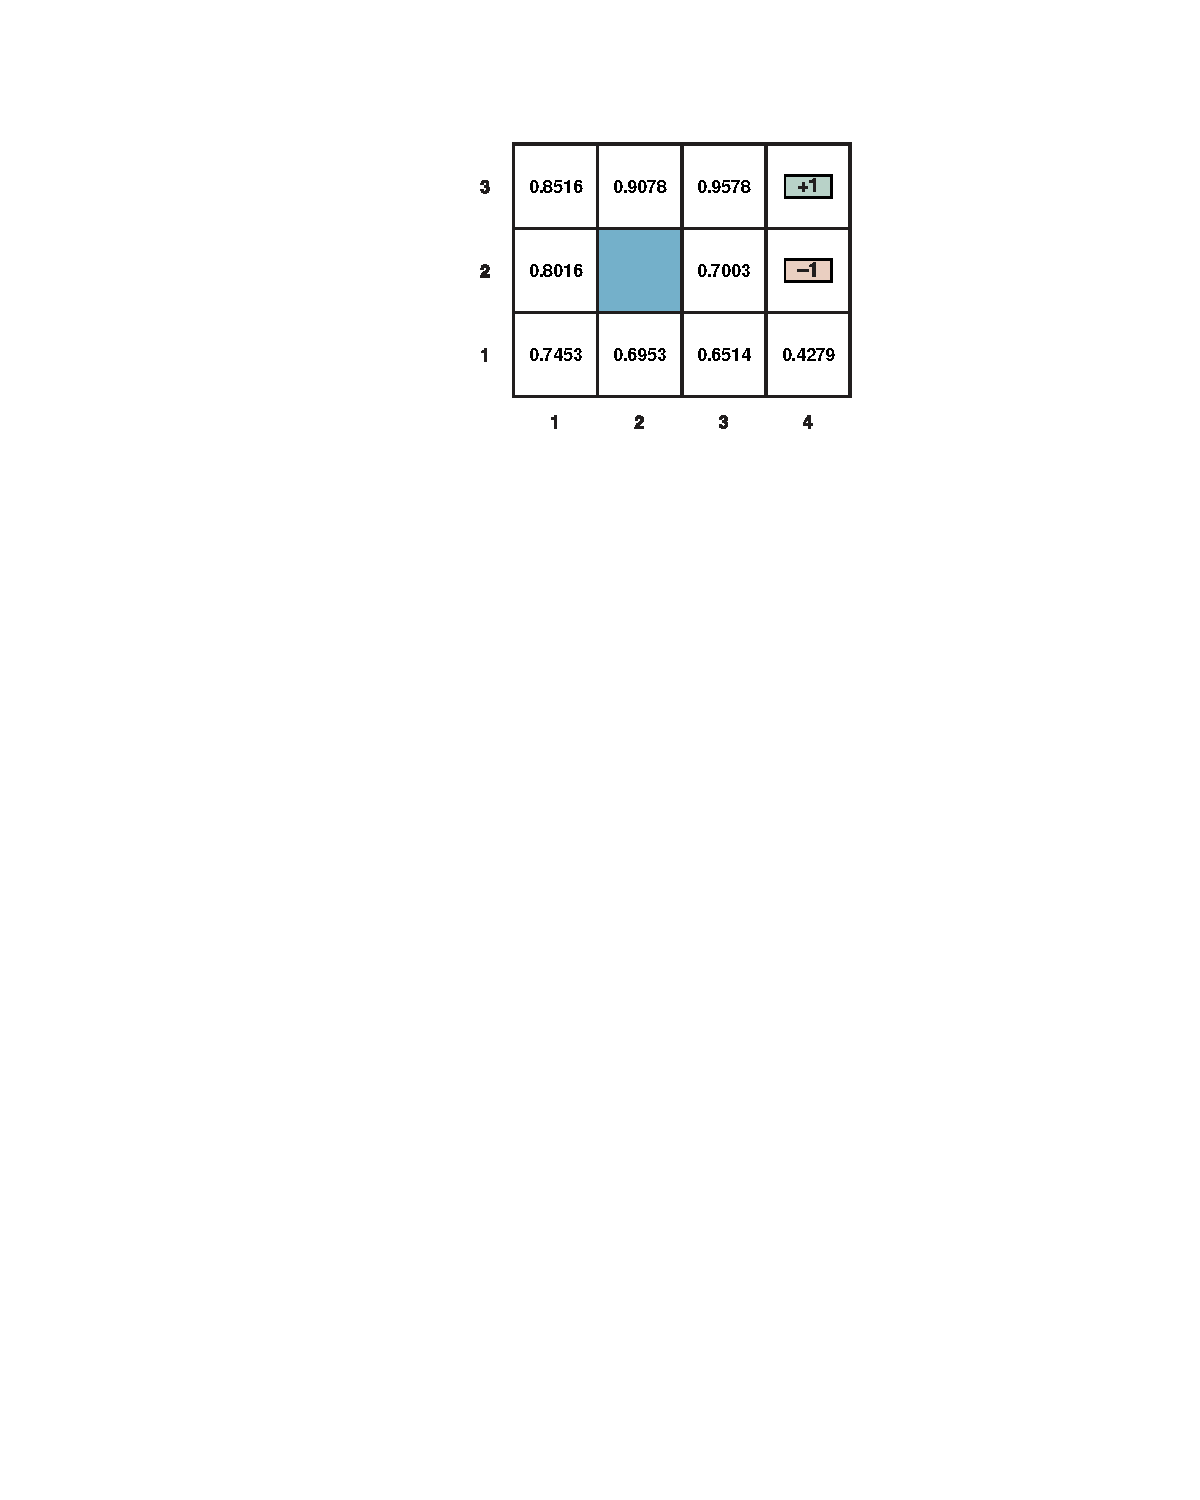
\includegraphics[alt={aima fig 17_03 state values},height=1.6in]{aima-fig-17_03-state-values.pdf}





We plug the state values above and \(\gamma = 1\) into:

\vspace{-.2in}
\begin{align*}
\max \Big( &[0.8(-0.04 + \gamma V(1,2)) + 0.1(-0.04 + \gamma V(2,1)) + 0.1(-0.04 + \gamma V(1,1))], \tag{Up} \\
            &[0.9(-0.04 + \gamma V(1,1)) + 0.1(-0.04 + \gamma V(1,2))], \tag{Left} \\
            &[0.9(-0.04 + \gamma V(1,1)) + 0.1(-0.04 + \gamma V(2,1))], \tag{Down} \\
            &[0.8(-0.04 + \gamma V(2,1)) + 0.1(-0.04 + \gamma V(1,2)) + 0.1(-0.04 + \gamma V(1,1))] \Big) \tag{Right}
\end{align*}

which yields \(Up\) as the optimal action because \(Up\) is the action that maximizes \(V((1, 1))\).
\section{Action Values and Optimal Policies}
\label{sec:org55f9933}

\begin{equation*}
V(s) = \max_{a} Q(s, a)
\end{equation*}

The optimal action value function is:

\[
Q^*(s_t, a_t ) = \max_{\pi} \big( \mathbb{E} [G_t | s_t, a_t^{\pi}] \big)
\]

If we know \(Q^*\) we can use it to derive an optimal policy, \(\pi^*\):

\[
\pi^*(a_t | s_t ) \leftarrow \argmax_{a_t} \left( Q^*(s_t, a_t ) \right)
\]

We'll see this idea when we solve MDPs using dynamic programming.
\section{Optimal Policies}
\label{sec:orgec607d6}

Notice that in State (3, 1) there are two optimal actions:


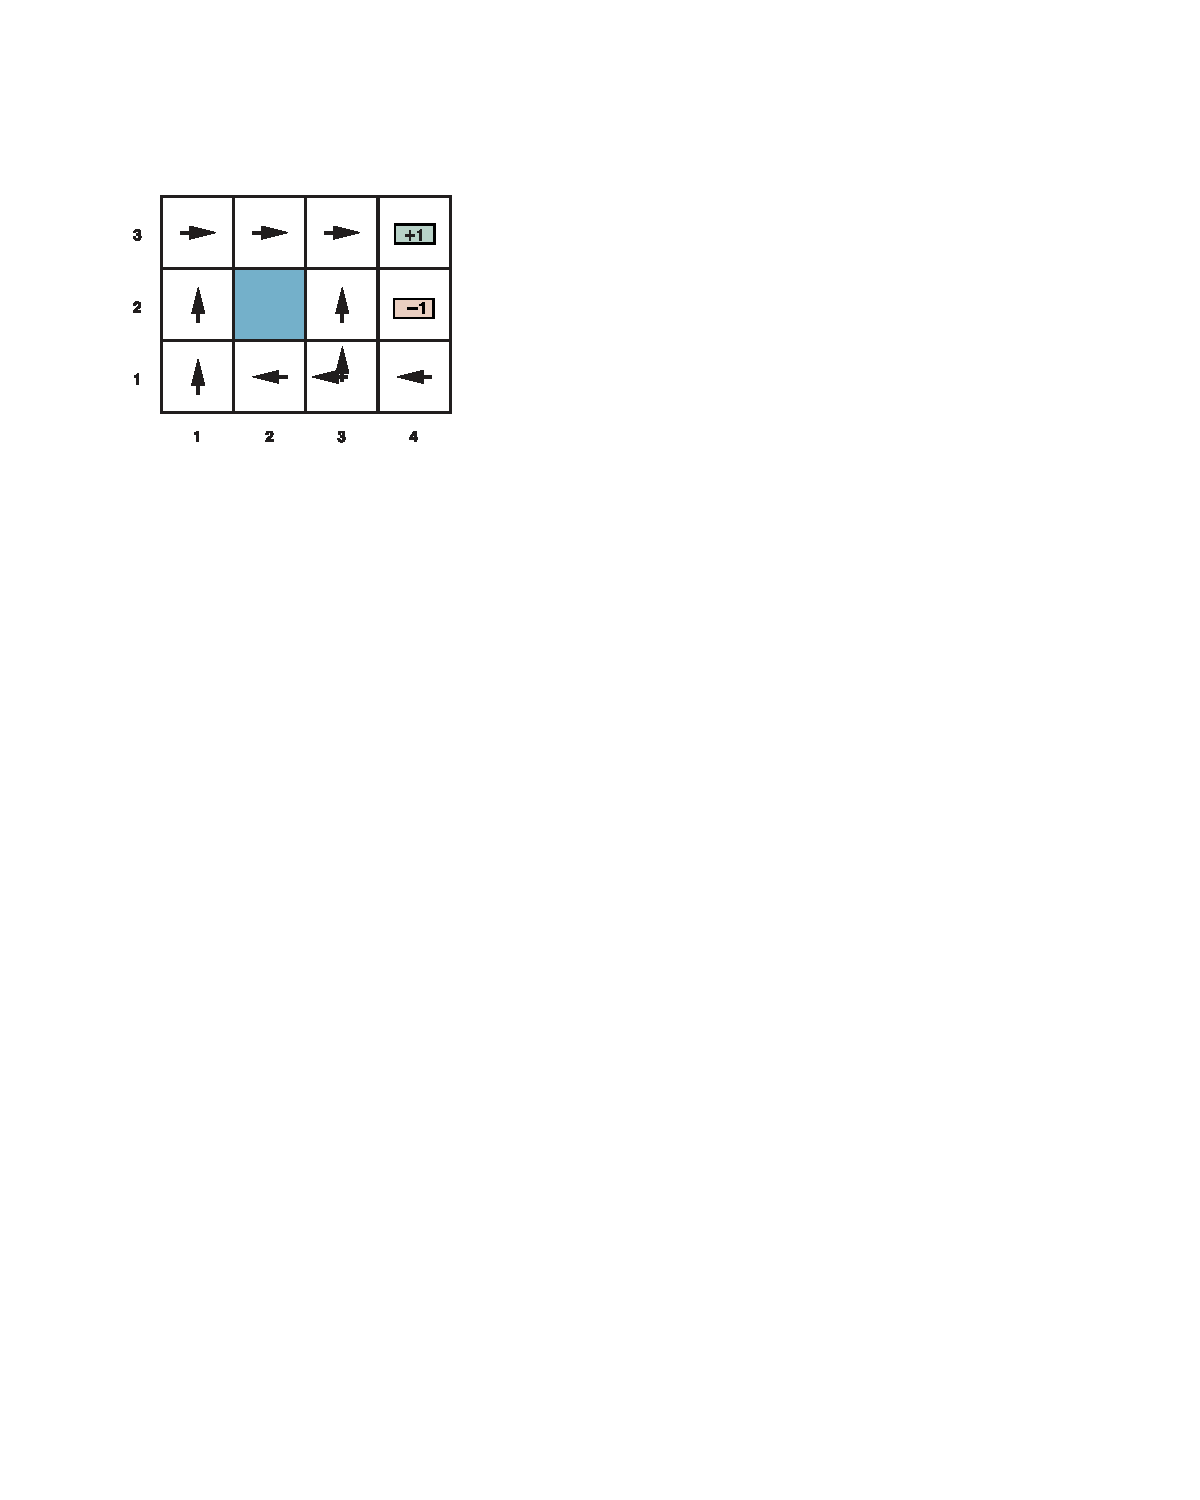
\includegraphics[alt={aima fig 17_02_a optimal policies},width=0.75\linewidth]{aima-fig-17_02_a-optimal-policies.pdf}


This results from the successor states having equal values, giving rise to multiple optimal policies.
\section{Reward Structures}
\label{sec:org7335437}

Notice how different reward structures for non-goal states influences the optimal policy:


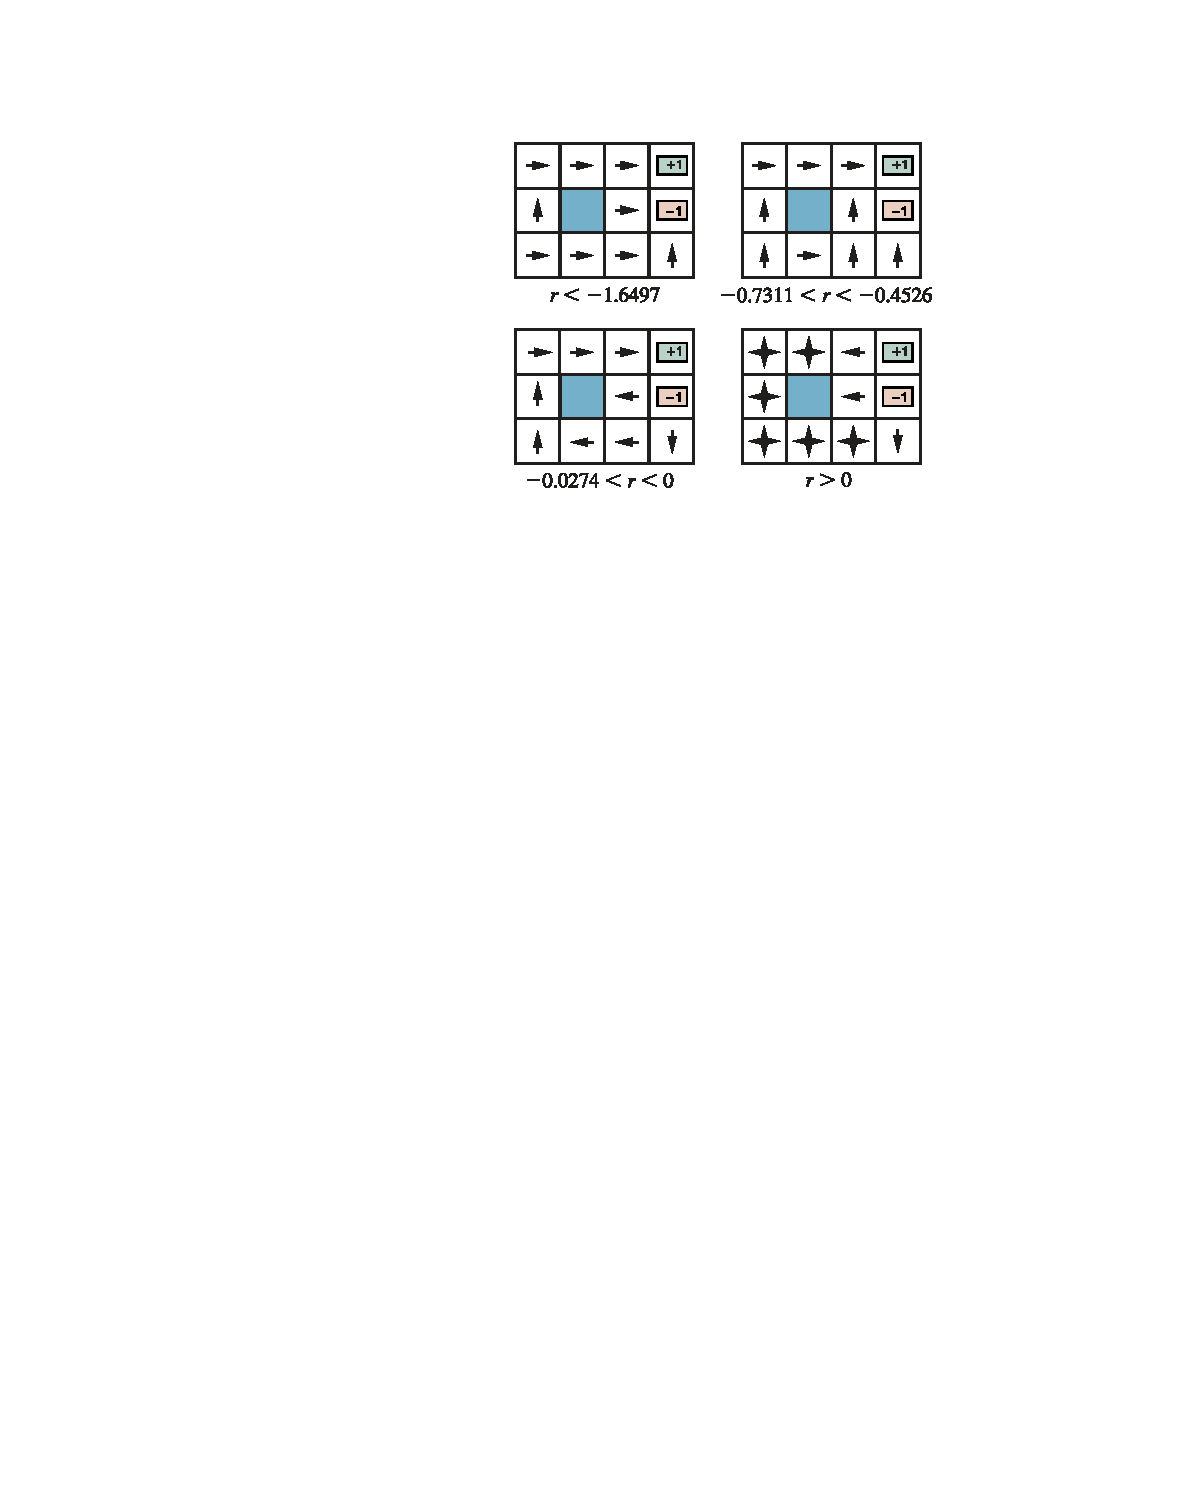
\includegraphics[alt={aima fig 17_02_b optimal policies different rewards},width=0.75\linewidth]{aima-fig-17_02_b-optimal-policies-different-rewards.pdf}


In general, negative rewards "motivate" the agent to seek the goal quickly.
\section{Representing MDPs}
\label{sec:orgca019f0}


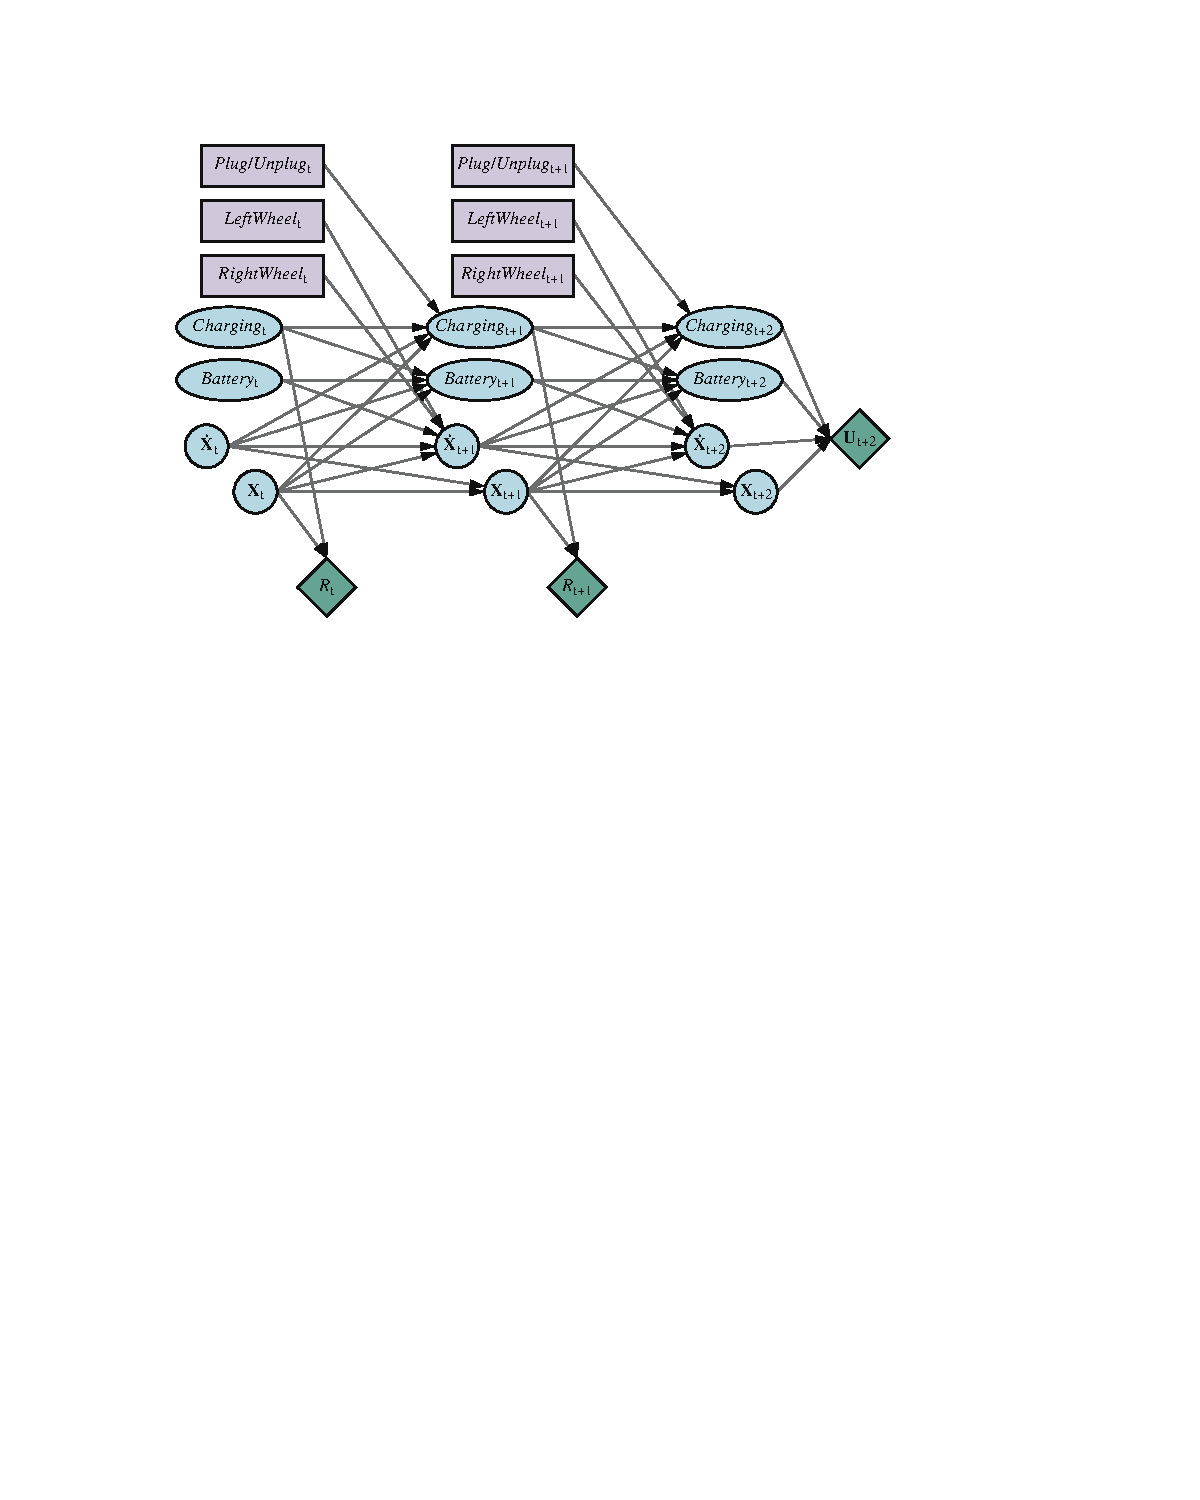
\includegraphics[alt={aima fig 17_04 decision network robot mdp},width=0.75\linewidth]{aima-fig-17_04-decision-network-robot-mdp.pdf}
\section{Bellman Value Update Rule}
\label{sec:org8285a14}

The value iteration algorithm initializes each state's value to a random value, then iteratively update these values by turning the Bellman equation into an update rule (the Bellman update):

\begin{equation}\label{eqn:bellman-update}
V_{i+1}(s) \leftarrow R(s) + \max_{a \in A} \sum_{s'} T(s, a, s') V_i(s')
\end{equation}

These updates are applied at the same time for all states, i.e., the values in iteration \(i+1\) are calculated from the values in iteration \(i\). The value iteration algorithm is shown in Algorithm \ref{alg:value-iteration}.

\begin{algorithm}[H]
  \caption{Value Iteration}\label{alg:value-iteration}
  \begin{algorithmic}
    \State $V \gets$ random initial values
    \Repeat
      \State $V' \gets V$
      \For{each $s \in S$}
        \State $V'(s) \gets R(s) + \max_{a \in A} \sum_{s'} T(s, a, s') V(s')$
      \EndFor
      \State $V \gets V'$
    \Until $V$ changes by a sufficiently small amount
  \end{algorithmic}
\end{algorithm}
\section{Value Iteration Algorithm}
\label{sec:org99a6e18}


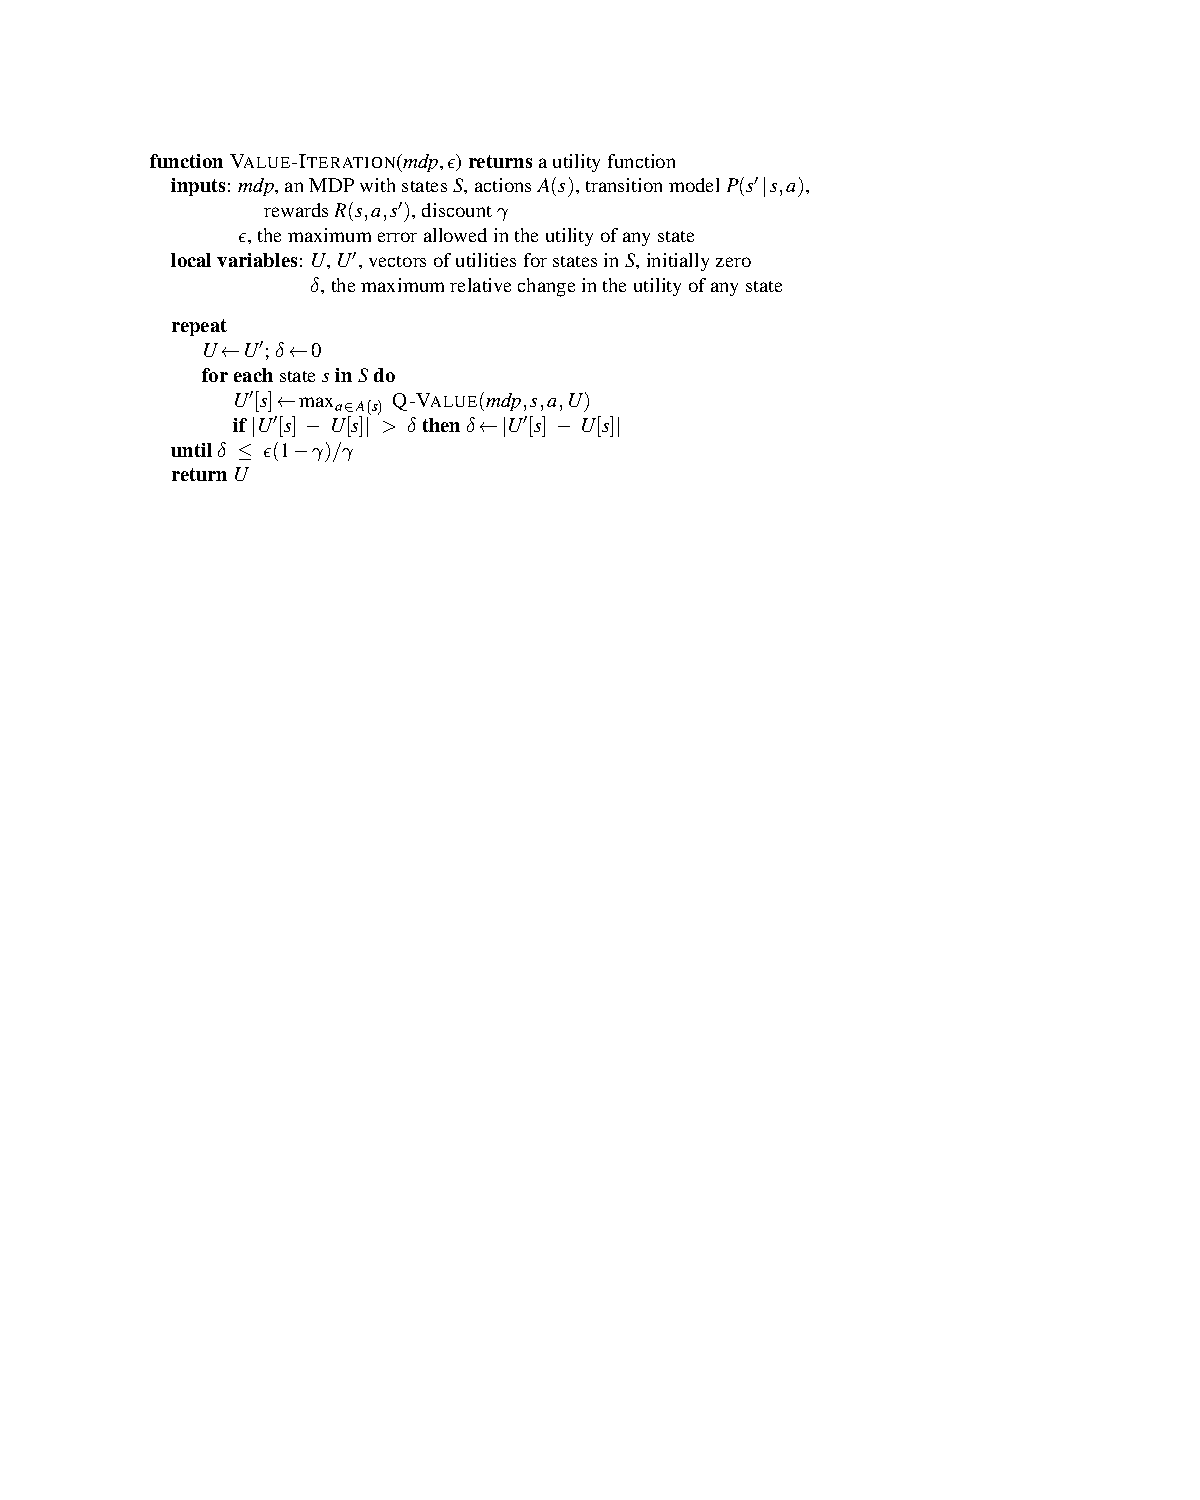
\includegraphics[alt={aima fig 17_06 value iteration algorithm},width=0.75\linewidth]{aima-fig-17_06-value-iteration-algorithm.pdf}
\section{Value Iteration Converges Quickly}
\label{sec:org9caf8c4}


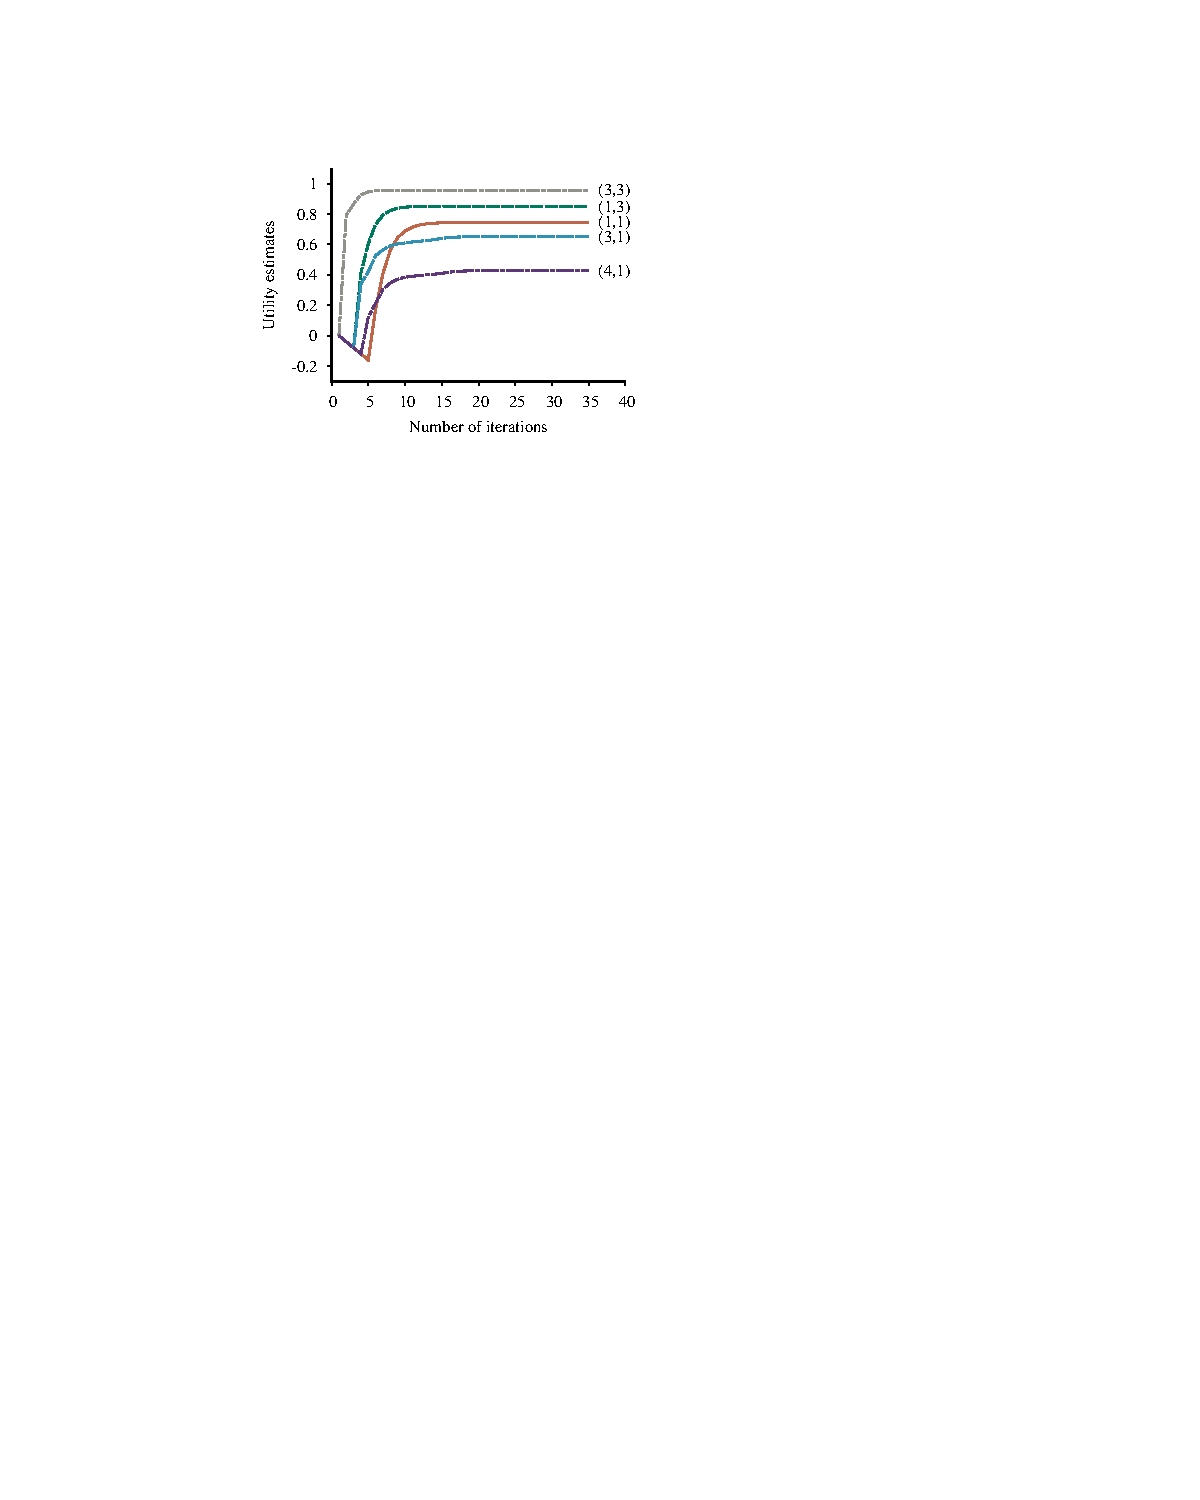
\includegraphics[alt={aima fig 17_07_a value estimates vs iterations plot},width=0.75\linewidth]{aima-fig-17_07_a-value-estimates-vs-iterations-plot.pdf}
\section{Policy Iteration}
\label{sec:org2260540}

In policy iteration \cite{howard1960dynamic} we start with a random initial values and policy and alternate between two steps for each iteration \(i\):

\begin{itemize}
\item \textbf{Policy evaluation.} Use policy \(\pi_i\) to calculate the values of each state using the discounted current values of their successor states. Since we are calculating the values under a particular policy, we drop the \(\max\) operator:

\begin{equation}
V_{i+1}(s) = R(s) + \gamma \sum_{s'} T(s, a, s') V(s')
\end{equation}

\item \textbf{Policy improvement.} Calculate policy \(\pi_{i+1}\) using the values calculated in the previous step.
\end{itemize}

When policy improvement does not change the policy, an optimal policy has been found and policy iteration terminates.

Note that since the update equation used in policy evaluation is linear, we can use linear algebra to solve the set of simultaneous linear equations in \(O(n^3)\). This method works fine for smaller state spaces but may be too expensive for large state spaces. A solution to this problem is known as modified policy iteration \cite{van-nunen1976set,puterman1978modified}, which combines policy iteration with value iteration by using a bounded number of Bellman updates to perform the policy evaluation step.
\section{Policy Iteration Algorithm}
\label{sec:orgb16c0a6}


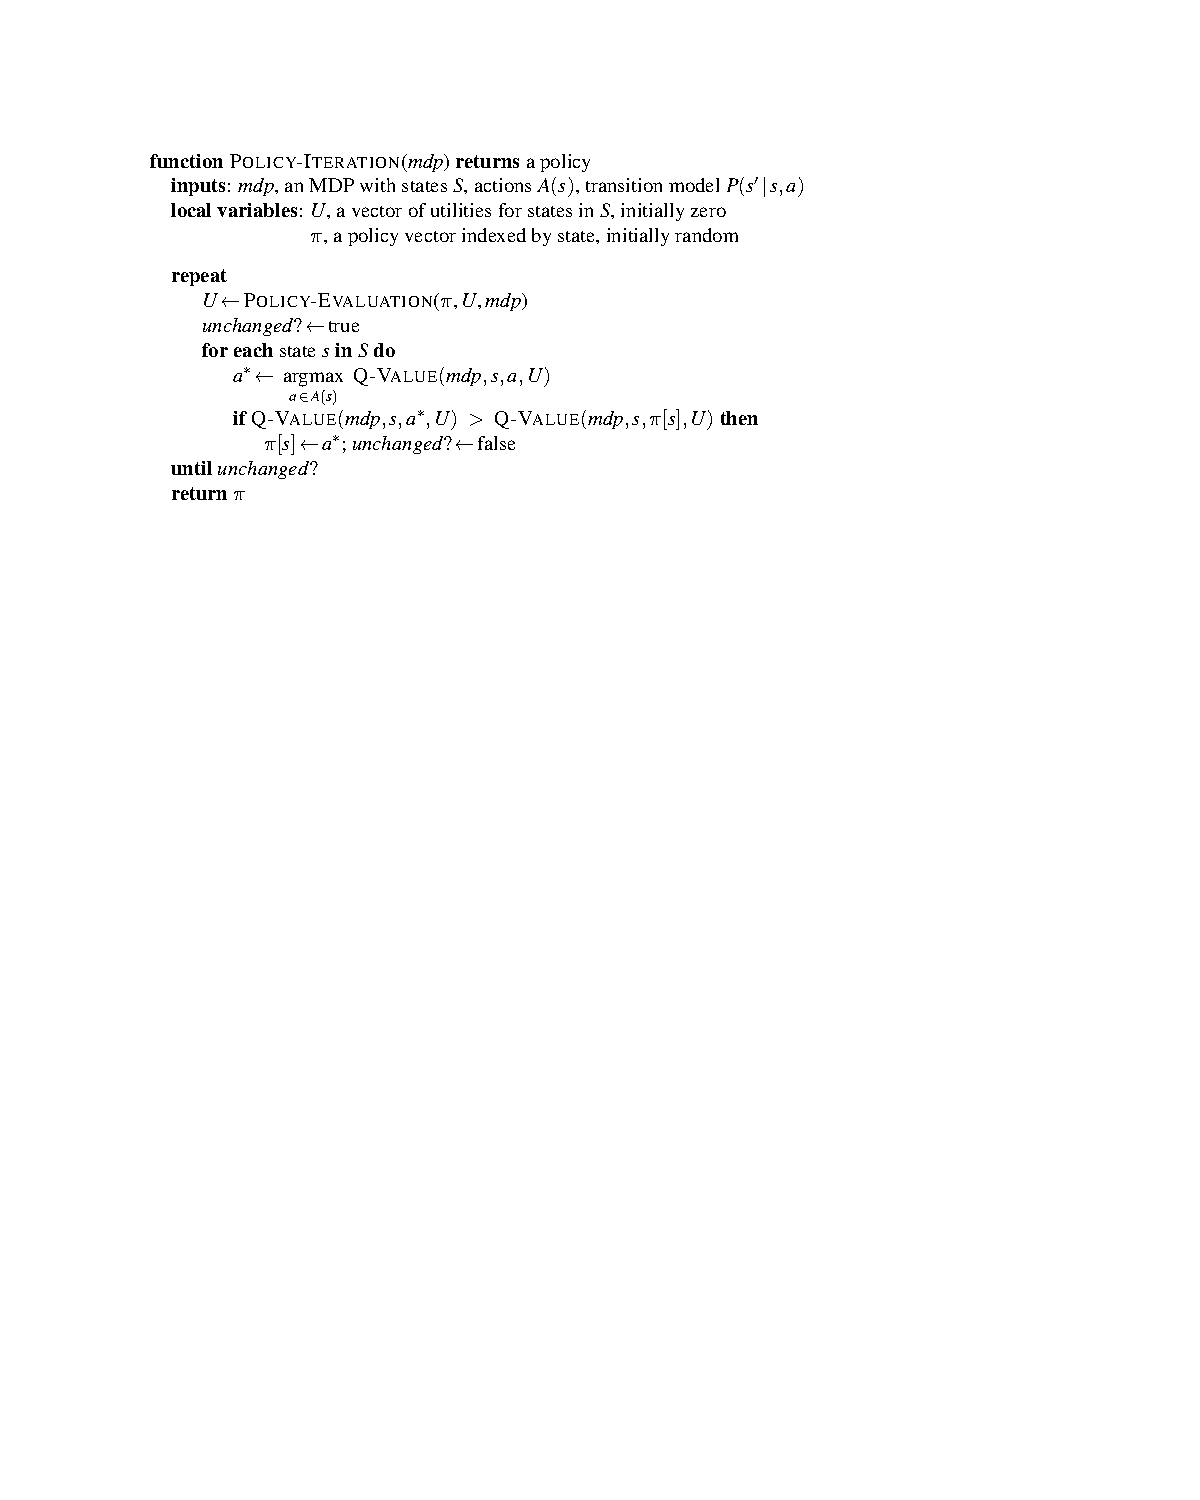
\includegraphics[alt={aima fig 17_09 policy iteration algorithm},width=0.75\linewidth]{aima-fig-17_09-policy-iteration-algorithm.pdf}
\section{\$k\$-Armed Bandits}
\label{sec:orgc20a411}

In Las Vegas, a \textbf{one-armed bandit} is a slot machine with one.  A \$k\$-armed bandit is \(k\) levers, each of which gives a sequence of rewards according to an unknown probability distribution. Problem: which arm should agent pull next?




Many practical applications:

\begin{itemize}
\item deciding between \(k\) treatments to cure a disease,
\item deciding between \(k\) investments,
\item deciding between \(k\) research projects to fund,
\item deciding between \(k\) advertisements to show a web page visitor,
\item A/B testing.
\end{itemize}





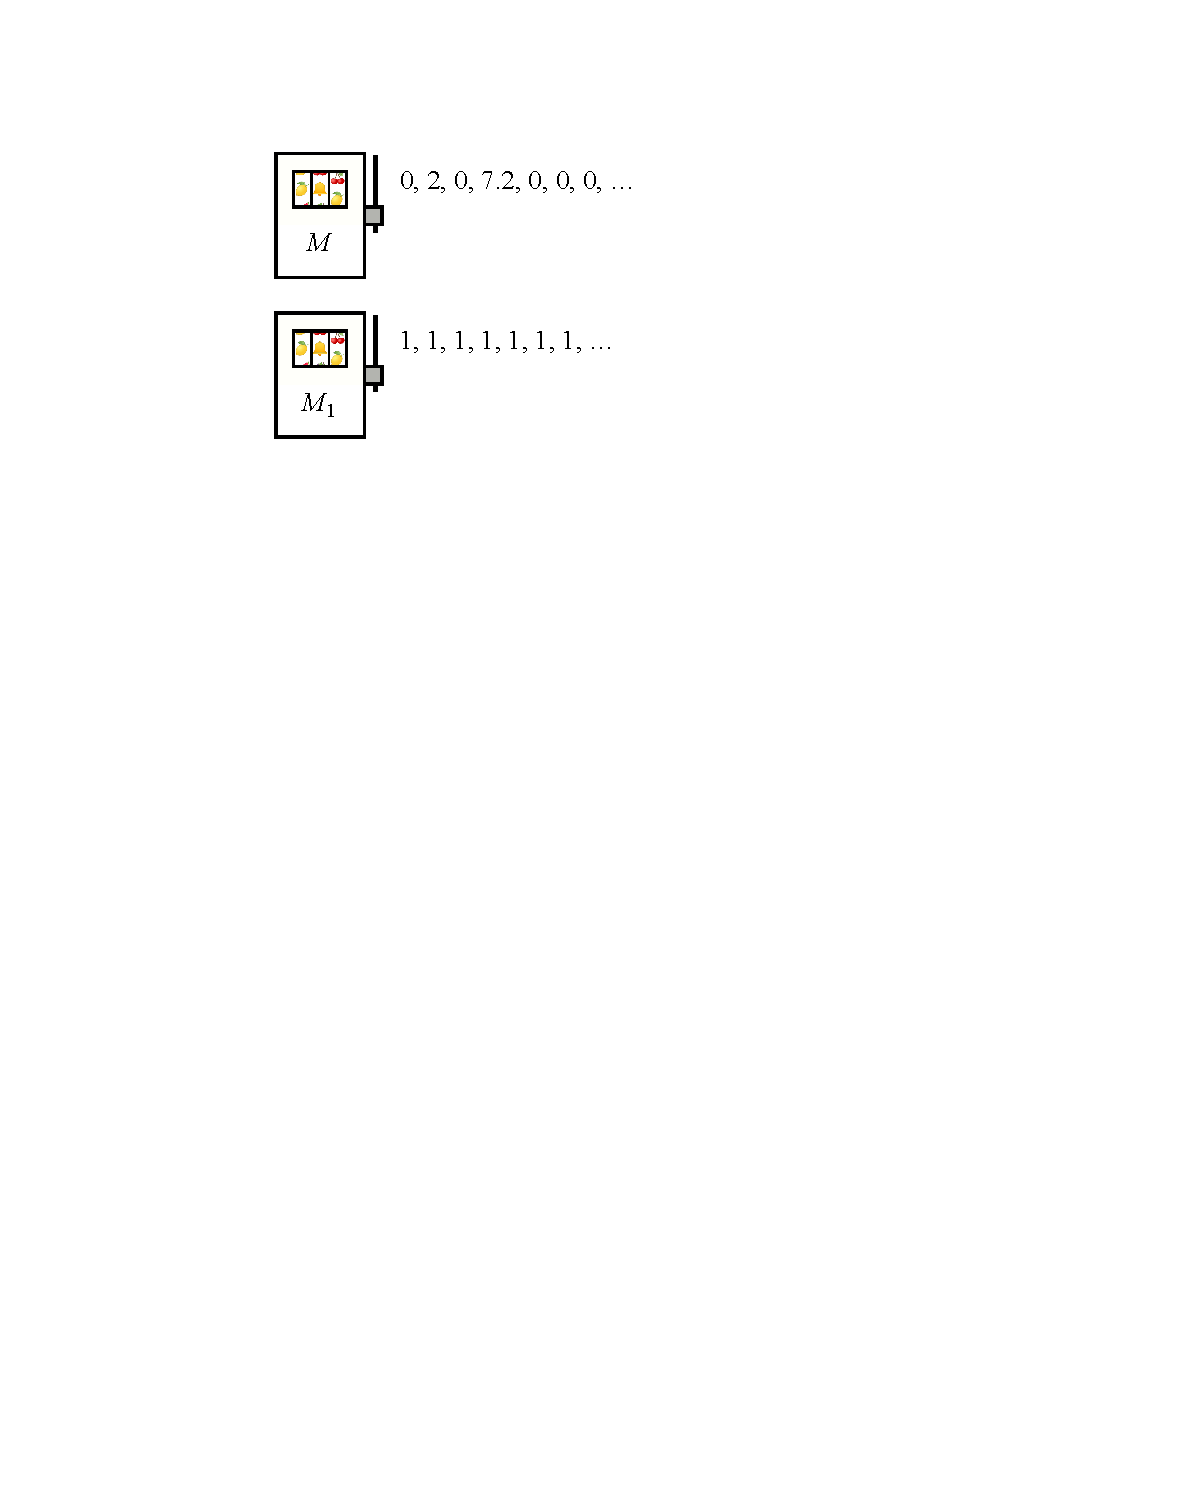
\includegraphics[alt={aima fig 17_12_a simple bandit},width=0.75\linewidth]{aima-fig-17_12_a-simple-bandit.pdf}
\section{Optimal Bandit Policy via Gittins Index}
\label{sec:orgbf4fdeb}




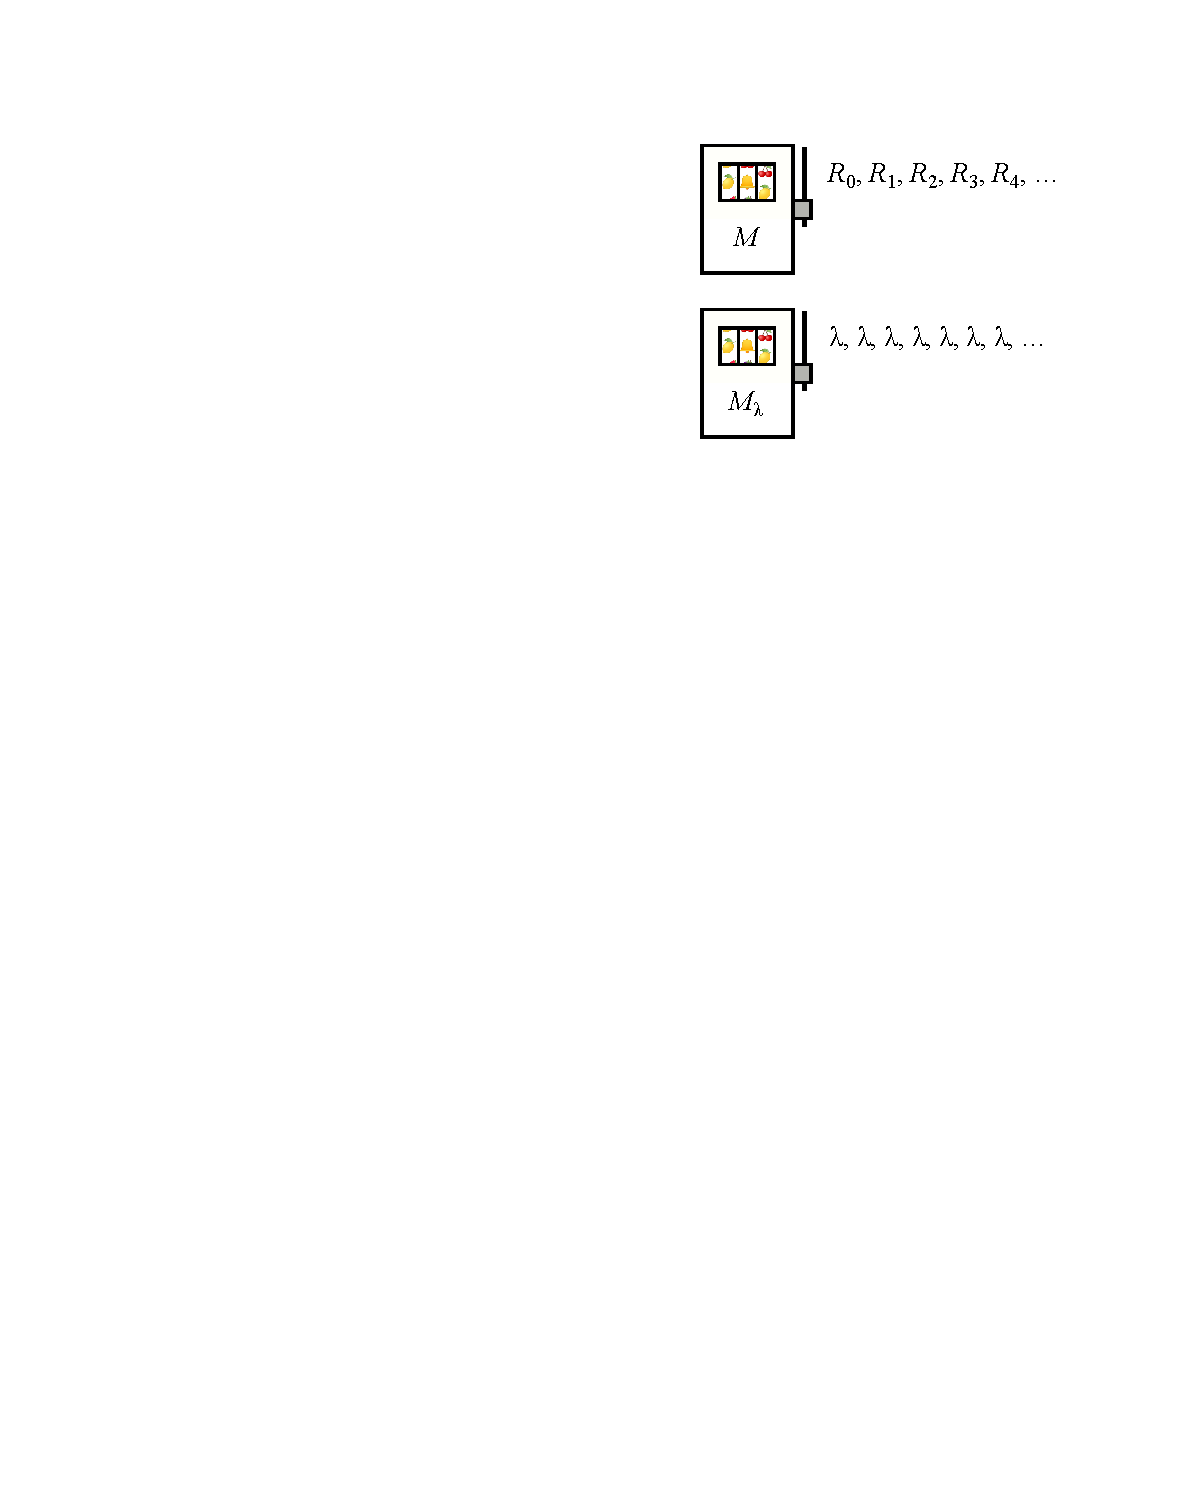
\includegraphics[alt={aima fig 17_12_b general bandit},width=0.75\linewidth]{aima-fig-17_12_b-general-bandit.pdf}




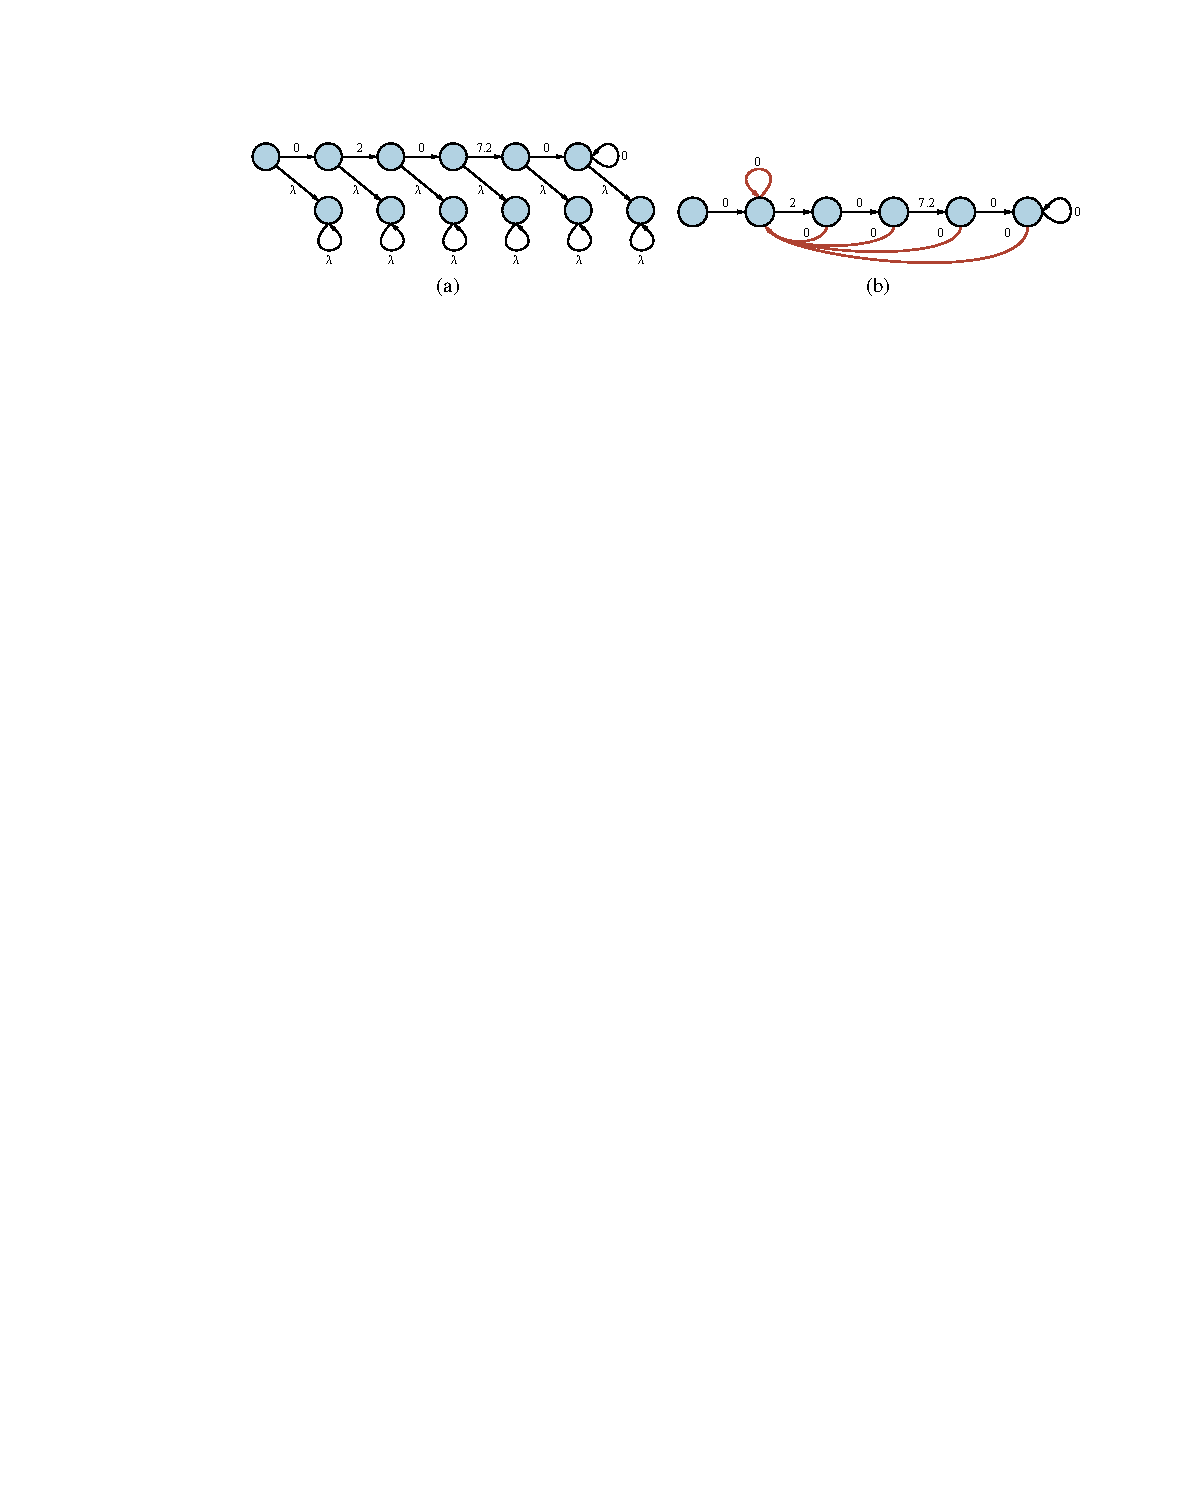
\includegraphics[alt={aima fig 17_13 switch mdp restart mdp},width=0.75\linewidth]{aima-fig-17_13-switch-mdp-restart-mdp.pdf}
\section{Bernoulli Bandit}
\label{sec:org2d08a76}









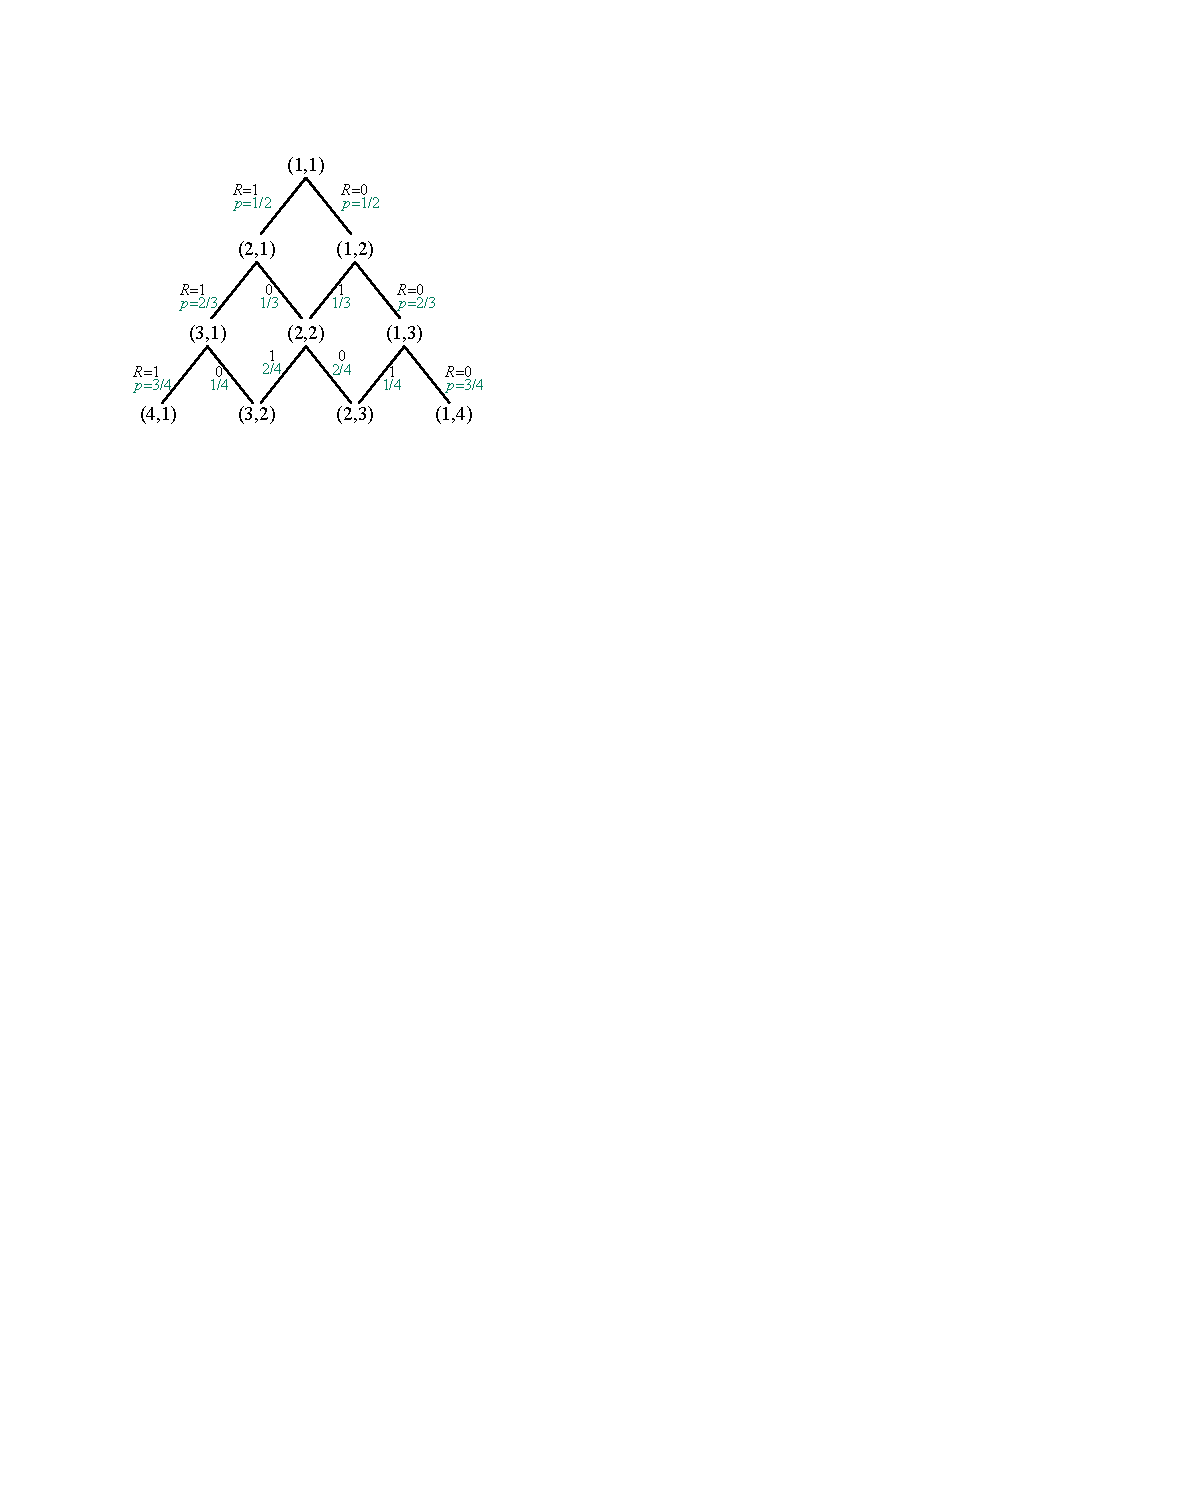
\includegraphics[alt={aima fig 17_14_a bernoulli bandit reward process},width=0.75\linewidth]{aima-fig-17_14_a-bernoulli-bandit-reward-process.pdf}
\section{Approximately Optimal Bandit Policies}
\label{sec:org74429e1}




\section{POMDP Value Iteration Algorithm}
\label{sec:orgb7d917f}


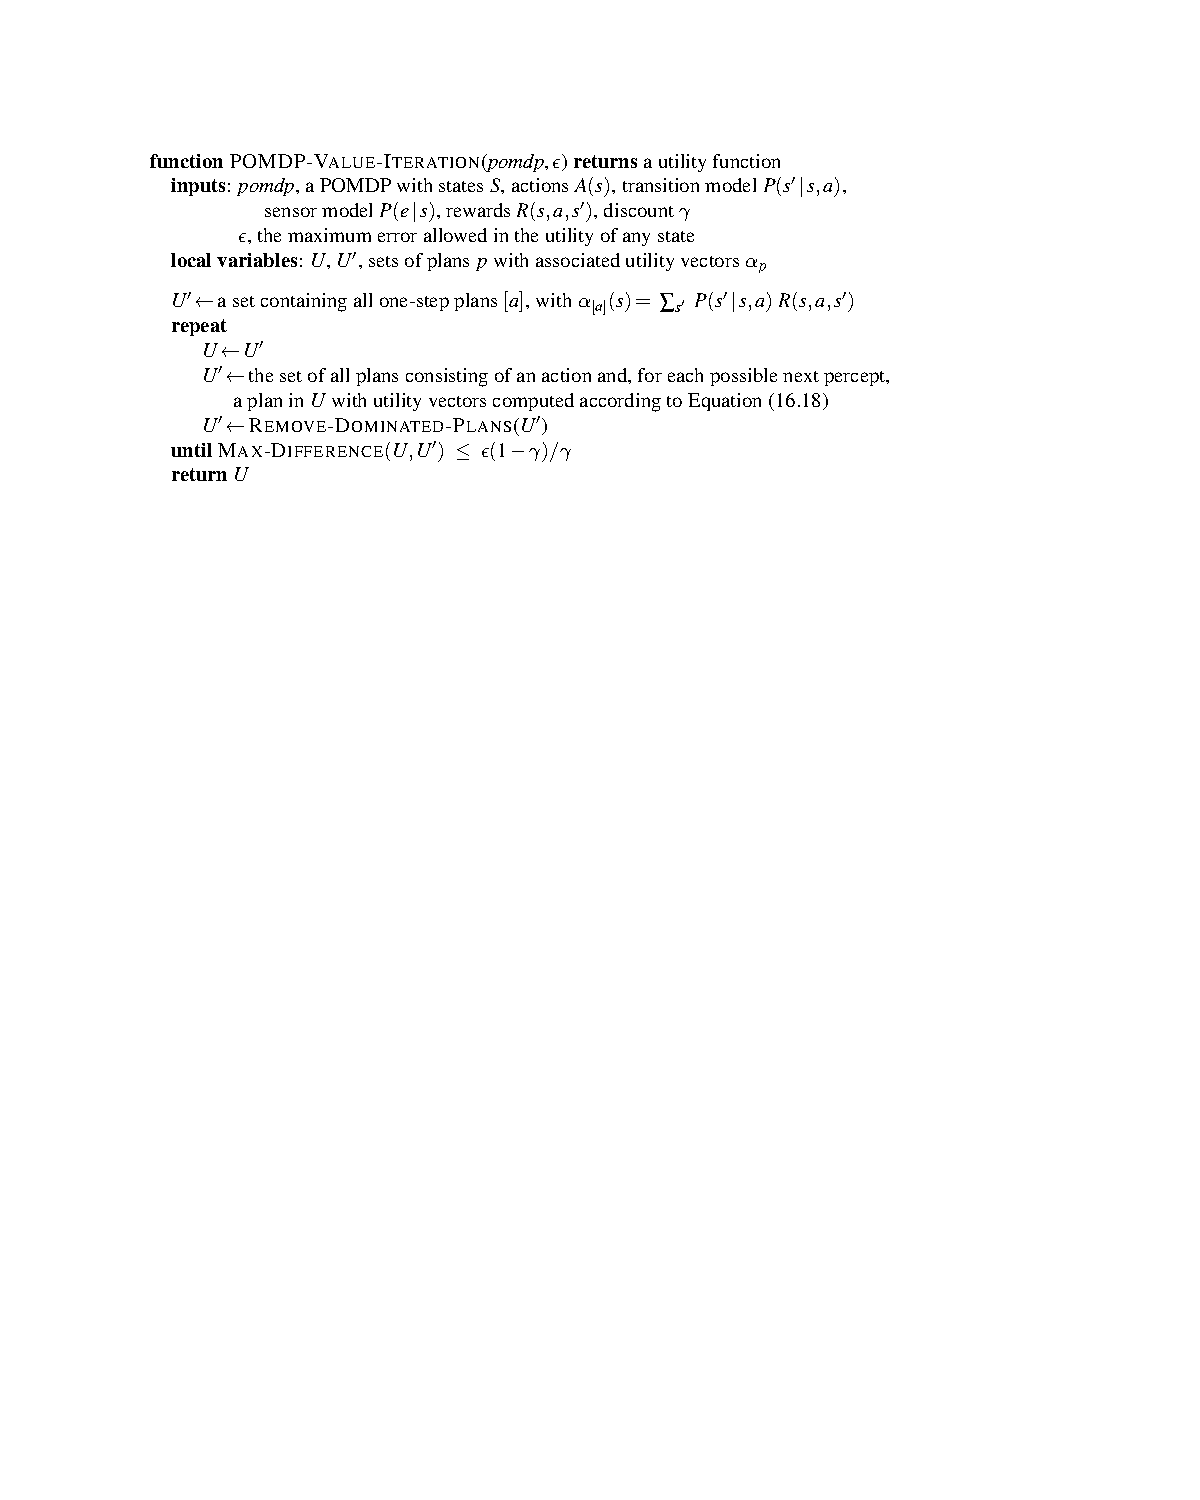
\includegraphics[alt={aima fig 17_16 pomdp value iteration algorithm},width=0.75\linewidth]{aima-fig-17_16-pomdp-value-iteration-algorithm.pdf}
\section{Online POMDP Algorithms}
\label{sec:org3e0c777}


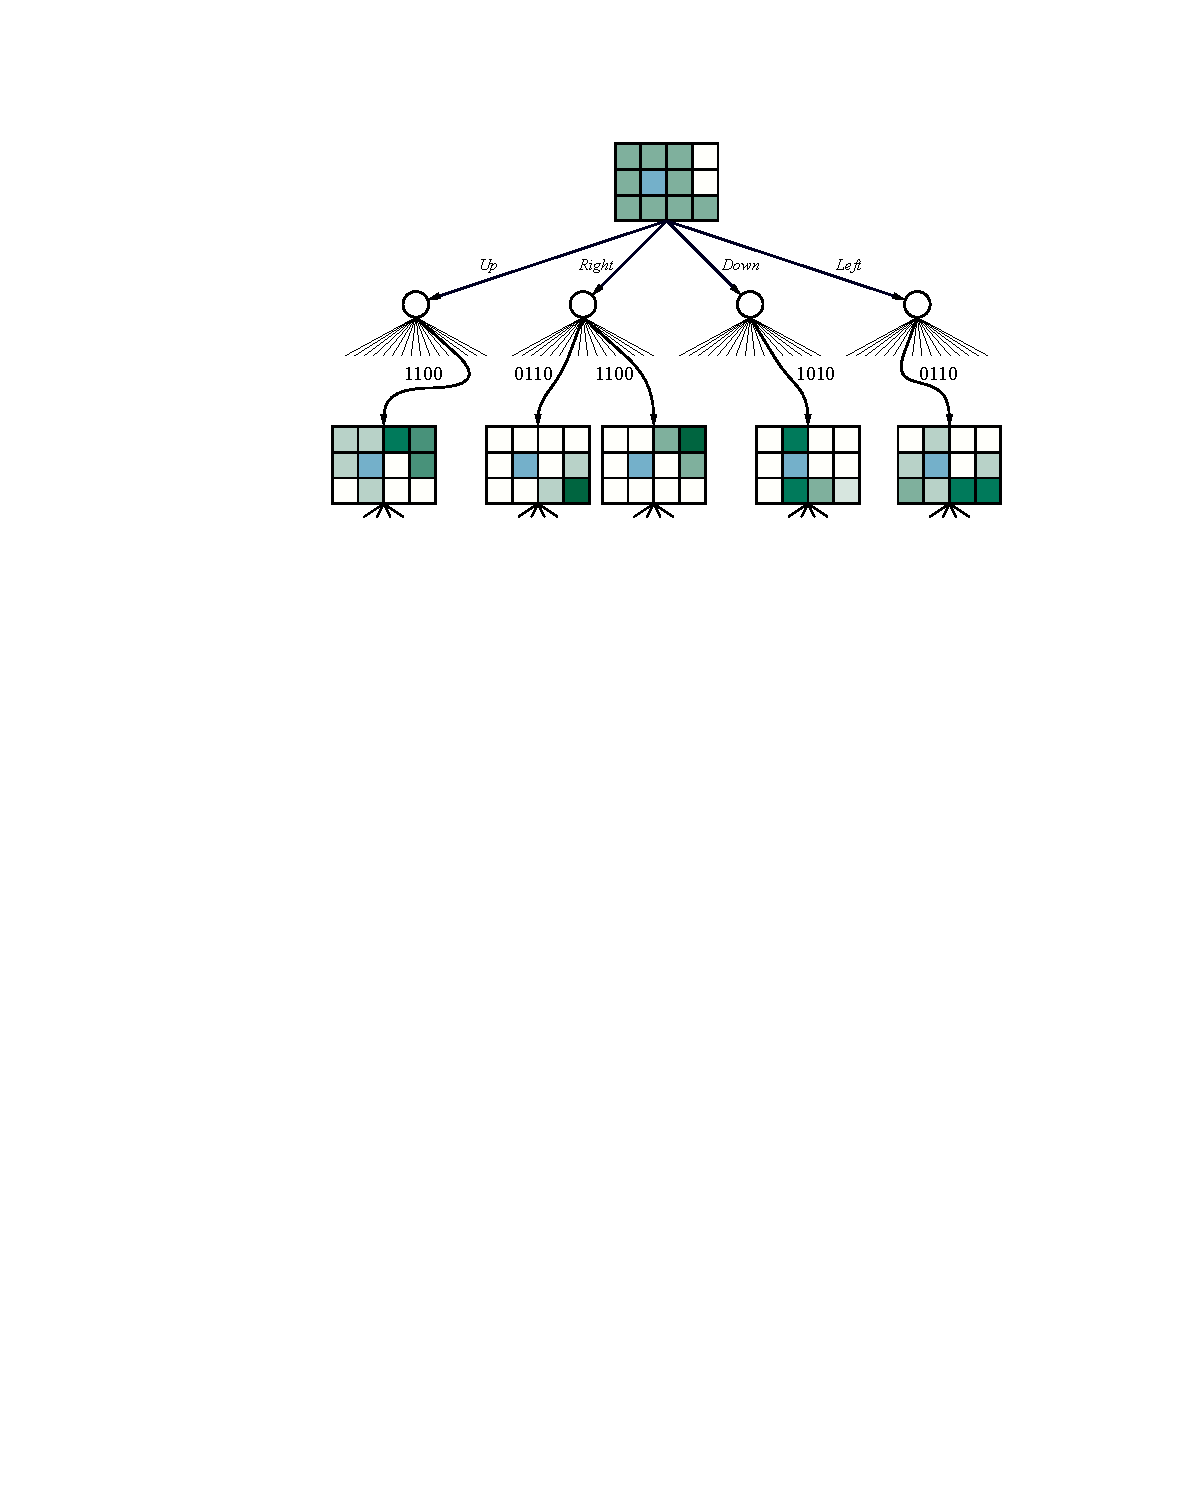
\includegraphics[alt={aima fig 17_17 pomdp expectimax tree},width=0.75\linewidth]{aima-fig-17_17-pomdp-expectimax-tree.pdf}
\section{POMDP Belief Updates}
\label{sec:org2ac1c92}


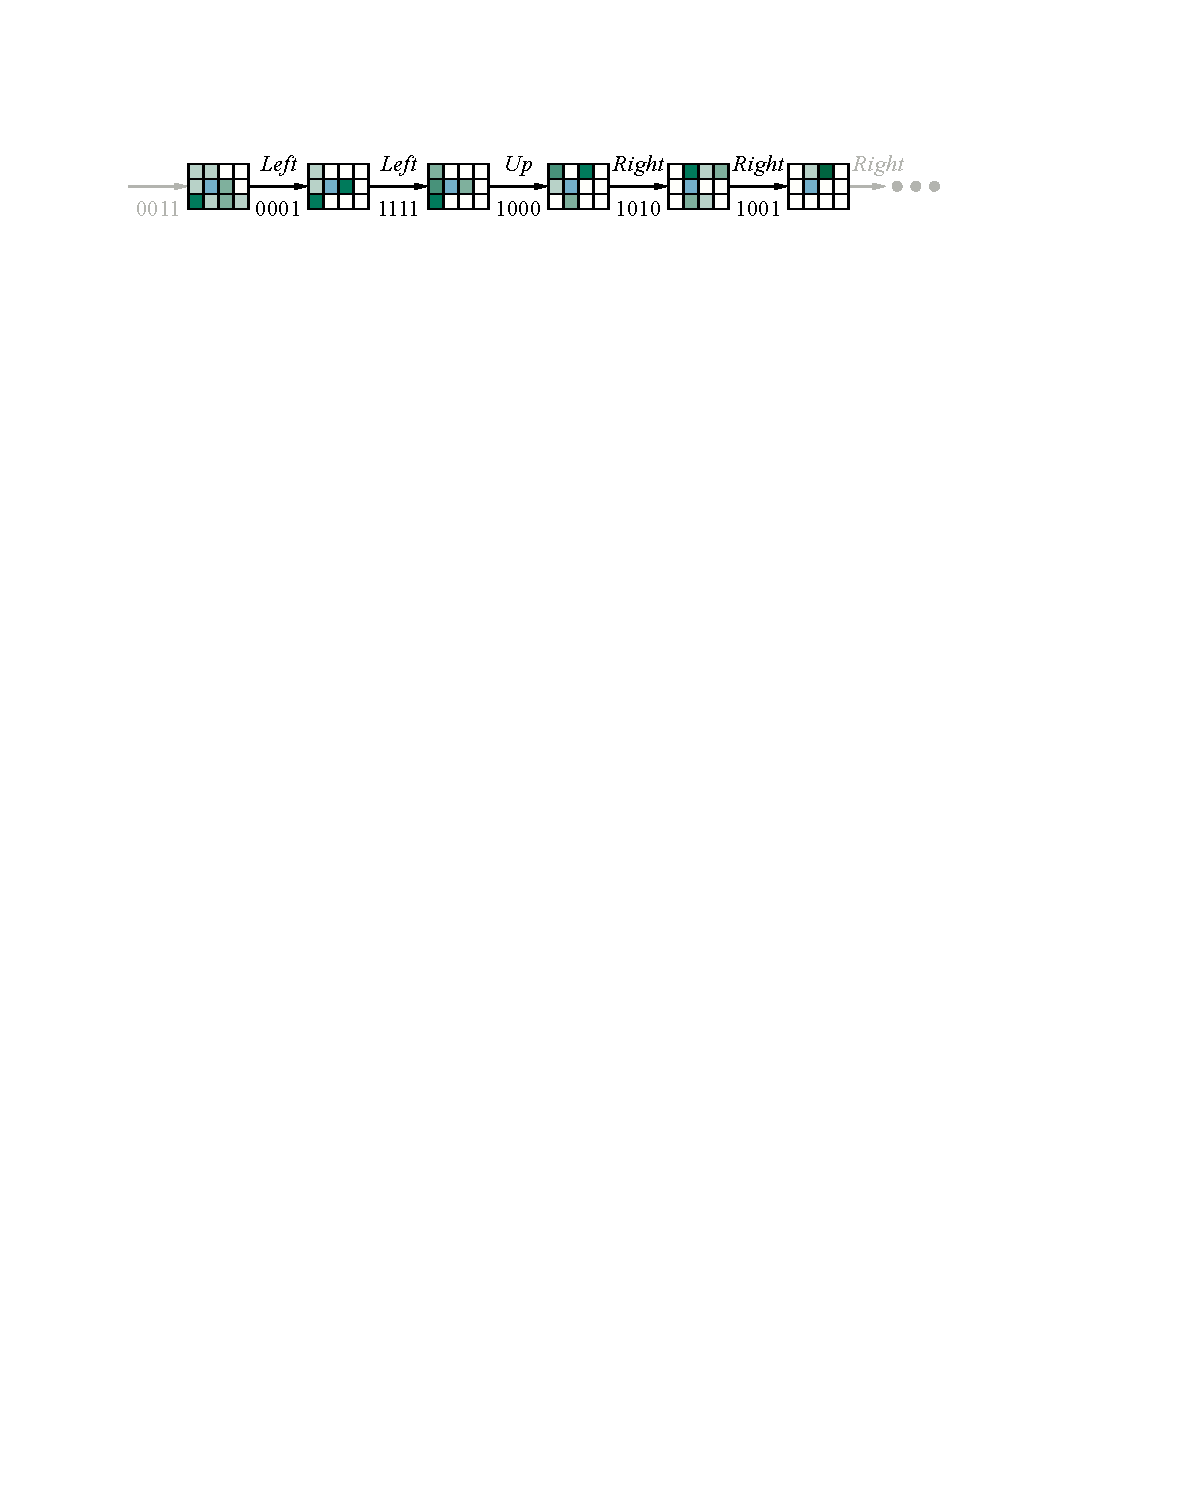
\includegraphics[alt={aima fig 17_18 pomdp belief state sequence},width=0.75\linewidth]{aima-fig-17_18-pomdp-belief-state-sequence.pdf}
\end{document}
